\documentclass[10pt,xcolor=table]{beamer}

\usetheme[progressbar=frametitle]{metropolis}
\usepackage{appendixnumberbeamer}
\usepackage{hyperref}

\newcommand{\verbatimfont}[1]{\renewcommand{\verbatim@font}{\ttfamily#1}}

\newcommand{\PR}[1]{\ensuremath{\left[#1\right]}}
\newcommand{\PC}[1]{\ensuremath{\left(#1\right)}}
\newcommand{\chav}[1]{\ensuremath{\left\{#1\right\}}}

\usepackage{booktabs}
\usepackage[scale=2]{ccicons}

\usepackage{pgfplots}
\usepgfplotslibrary{dateplot}

\usepackage{xspace}
\newcommand{\themename}{\textbf{\textsc{metropolis}}\xspace}

\setbeamertemplate{frame footer}{
\includegraphics[height=0.7cm]{figuras/ifpb.png}}

\setbeamercolor{background canvas}{bg=white}

\title{Redes sem Fio}
\subtitle{Redes sem Fio - Apresentação da Disciplina}
% \date{\today}
\date{}
\author{Prof. Ruan Delgado Gomes}
\institute{UA2 - IFPB}
\titlegraphic{\hfill
\includegraphics[height=2cm]{figuras/ifpb.png}}


\begin{document}

\maketitle

\begin{frame}
	\frametitle{Motivação}
    \begin{block}{Por que estudar Redes sem Fio?}
		\begin{itemize}
			\item Tecnologia \textbf{amplamente utilizada} em \textbf{diferentes contextos}
            \vspace{2mm}
            \item \textbf{Desafios únicos} relacionados à \textbf{transmissão de sinais sem fio}
            \vspace{2mm}
            \item Protocolos e mecanismos \textbf{específicos} na camada de enlace
		\end{itemize}
	\end{block}
	\begin{figure}[htbp]
    	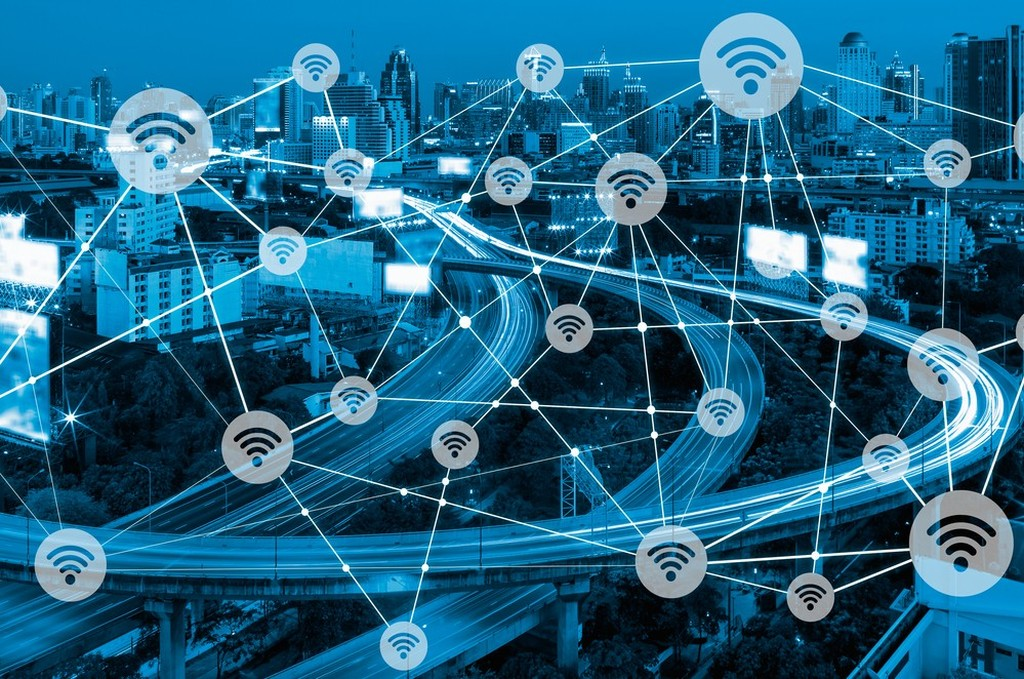
\includegraphics[width=0.5\textwidth]{figuras/WirelessNetwork-1.jpg}\\
        \tiny fonte: \url{https://predictabledesigns.com/wireless_technologies_bluetooth_wifi_zigbee_gsm_lte_lora_nb-iot_lte-m/}. Acesso em 15/02/2024.
	\end{figure}
\end{frame}

\begin{frame}
	\frametitle{Histórico}
    \begin{block}{Comunicações sem fio não é algo novo}
		\begin{itemize}
			\item Telégrafo sem fio - primeira transmissão de longa distância feita em 1901
            \vspace{2mm}
            \item Comunicações via satélite - início em 1960
            \vspace{2mm}
            \item Telefonia celular - primeira rede 1G lançada em 1979
            \vspace{2mm}
            \item Redes locais sem fio - primeiro padrão IEEE 802.11 lançado em 1997
            \vspace{2mm}
            \item Redes de sensores - primeiro padrão IEEE 802.15.4 lançado em 2003
		\end{itemize}
	\end{block}
\end{frame}

\begin{frame}
\frametitle{Histórico}
    Alguns marcos em comunicações sem fio\\
    \vspace{2mm}
	\begin{figure}[htbp]
    	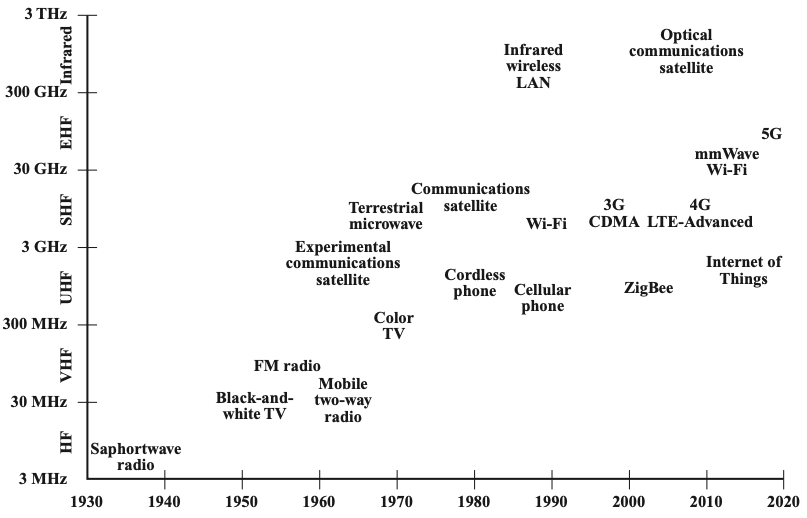
\includegraphics[width=0.9\textwidth]{figuras/milestonesredessemfio.png}\\
     	\tiny fonte: Stallings, William. Wireless communication networks and systems / William Stallings, Cory Beard, University of Missouri-Kansas City.First edition.
	\end{figure}
\end{frame}

\begin{frame}
\frametitle{Histórico}
    \begin{block}{A tecnologia de comunicações sem fio \textbf{continua avançando}}
		\begin{itemize}
            \item Redes 5G/6G
            \vspace{1mm}
            \item Wi-Fi 6/7
            \vspace{1mm}
            \item Novos padrões para IoT
		\end{itemize}
	\end{block}
    \begin{alertblock}{Vários desafios existem}
		\begin{itemize}
			\item Meio de comunicação ``não confiável''
            \begin{itemize}
                \item Desafios de propagação
                \vspace{1mm}
                \item Interferência
                \vspace{1mm}
                \item Co-existência
            \end{itemize}
            \item Espectro de comunicação \textbf{limitado}
            \vspace{2mm}
            \item Novas técnicas são criadas para \textbf{lidar com os desafios} e usar o espectro de maneira \textbf{mais eficiente}
		\end{itemize}
	\end{alertblock}
\end{frame}

\begin{frame}
	\frametitle{Sobre a Disciplina}
        \begin{block}{\small Principais Objetivos}
    		\begin{itemize}
    			\item \small Entender os conceitos sobre \textbf{transmissão de sinais sem fio}
                \vspace{1mm}
                \item \small Compreender os \textbf{efeitos de propagação} e como isso \textbf{influencia a qualidade de comunicação}
                \vspace{1mm}
                \item \small  Entender os conceitos sobre \textbf{protocolos de acesso ao meio} em redes sem fio
                \vspace{1mm}
                \item \small  Conhecer os mecanismos utilizados em \textbf{redes locais sem fio} (IEEE 802.11)
                \vspace{1mm}
                \item \small  Aprender a \textbf{planejar a implantação} de redes locais sem fio (IEEE 802.11)
                \vspace{1mm}
                \item \small  Conhecer as características de padrões para \textbf{redes sem fio de baixa potência} (ex: ZigBee, LoRa e \textit{Bluetooth})
                \vspace{1mm}
                \item \small  Conhecer a \textbf{arquitetura e as tecnologias} utilizadas em redes sem fio móveis (ex: redes 5G)
    		\end{itemize}
    	\end{block}
\end{frame}

\begin{frame}
	\frametitle{Sobre a Disciplina}
        \begin{block}{Formas de Avaliação}
    		\begin{itemize}
                \item Leitura prévia
                \vspace{2mm}
    			\item Minitestes valendo ponto (início e fim da aula)
                \vspace{2mm}
                \item Três provas discursivas
                \vspace{2mm}
                \item Experimento utilizando ESP32
    		\end{itemize}
    	\end{block}
\end{frame}

\begin{frame}
	\frametitle{Estudos para a Próxima Aula}
        \begin{block}{Realizar pesquisa em qualquer fonte (inclusive ferramentas de IA)}
    		\begin{itemize}
                \item Quais as vantagens e desvantagens das redes sem fio em comparação com as redes cabeadas?
                \vspace{2mm}
    			\item Quais os principais desafios das redes sem fio?
                \vspace{2mm}
                \item Quais os tipos de redes sem fio com relação à área de cobertura?
                \vspace{2mm}
                \item Quais as topologias usualmente utilizadas em redes sem fio?
                \vspace{2mm}
                \item Quais as principais diferenças entre as tecnologias de redes sem fio Wi-Fi, Bluetooth, ZigBee, LoRa e Redes 5G? Em que casos cada uma é mais aplicável?
    		\end{itemize}
    	\end{block}
\end{frame}

\end{document}

